\documentclass[12pt]{scrartcl}

\usepackage{amsmath, amssymb, amsthm, mathtools}

\usepackage{tikz, pgfplots}
\pgfplotsset{compat=1.17, width=10cm}
\usepgfplotslibrary{external}
\tikzexternalize

\usepackage[OT1]{fontenc}
\usepackage{mlmodern}
\usepackage{setspace}

\usepackage[backend=biber,style=numeric,sortcites=true]{biblatex}
\addbibresource{main.bib}

\usepackage{hyperref}

\graphicspath{ {./images/} }

\title{The Bigger The Better II}
\author{Group 8-29 \thanks{Derrick Lukimin (L, 2i204), Tan Yong Yih (2i222), Wu Hao (2i324), Darren Yap (2i425)}}
\date{2022}

\begin{document}
\onehalfspacing
\maketitle
\tableofcontents

\section{Introduction}
This project aims to find an algorithm to determine
the side length of the largest square that can be
inscribed inside a convex $n$-gon. It is a continuation from
a previous project completed in 2021, The Bigger The Better. \cite{tbtb1}

\subsection{Rationale}
Do note that the definition of inscribed is such that all vertices of the square lie on the sides of the polygon.

\subsection{Research Questions}
\begin{enumerate}
	\item What is the side length of the largest square that can be inscribed in a triangle?
	\item What is the side length of the largest square that can be inscribed in a regular $n$-gon, given $n \neq 4$?
	\item What is the side length of the largest square that can be inscribed in a convex $n$-gon?
\end{enumerate}

\subsection{Project Scope}
This project will mainly focus on polygons which are convex. This allows many restrictions to be made.

\section{Literature Review}
% stuff...

\section{Research Question 1}

\subsection{Introduction}
The first research question aims to find out the side length of the largest square that can be inscribed in a triangle, given the side lengths of the triangle.

\subsection{Key Insights}
\begin{enumerate}
	\item It can be seen that no more than 2 vertices of a square can lie on a single side, as a square has at most 2 vertices lying on a single line.
	\item We notice how a triangle has 3 sides, and a square has 4 vertices. In order for all the vertices to lie on the triangle, by pigeonhole principle, at least one side has at least 2 vertices lying on it.
	\item Combining the first 2 insights, we can see that 2 sides of the triangle will have 1 vertices each lying on it, while the other side will have 2 vertices lying on it.
\end{enumerate}

\subsection{Solutions}
A figure has been constructed for the purposes of illustrating the following proof.
\begin{figure}[htpb]
\centering
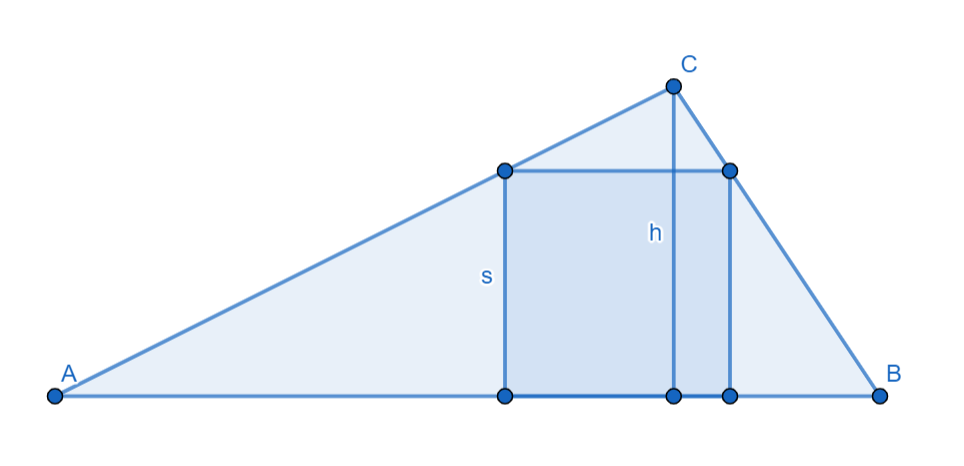
\includegraphics[scale=.75]{rq1}
\label{fig:rq1_img}
\caption{The figure for RQ1.}
\end{figure}

We see that side c can be formed with \(s\) as well as \(s \cot \angle A\) and \(s \cot \angle B\).
\begin{equation}
		c              & = s+s\cot \angle A+s\cot \angle B                                                                           \\
		s              & = \dfrac{c}{1+\cot \angle A+\cot \angle B}                                                                             \\
		               & = \dfrac{c \sin\angle A}{\sin\angle A+\cos\angle A+\cot\angle B\sin\angle A}                                        \\
		               & = \dfrac{c\sin\angle A\sin\angle B}{\sin\angle A\sin\angle B+\cos\angle A\sin\angle B+\sin\angle A\cos\angle B} \\
		               & = \dfrac{c\sin\angle A\sin\angle B}{\sin\angle A\sin\angle B+\sin\left(\angle A+\angle B\right)}                    \\
		               & = \dfrac{c\sin\angle A\sin\angle B}{\sin\angle A\sin\angle B+\sin\left(180-\angle C\right)}                         \\
		               & = \dfrac{c\sin\angle A\sin\angle B}{\sin\angle A\sin\angle B+\sin \angle C}                                         \\
		               & = \dfrac{2Rc\sin\angle A\sin\angle B}{2R\sin\angle A\sin \angle B+2R\sin \angle C}                                   \\
		               & = \dfrac{ac\sin\angle B}{a\sin\angle B+c}                                                                             \\
		               & = \dfrac{2Rac\sin\angle B}{2Ra\sin\angle B+2Rc}                                                                       \\
		               & = \dfrac{abc}{2Rc+ab}                                                                                                   \\
\end{equation}

Since each of the sides of the triangle, $a$, $b$ and $c$ can be the longest side, 
we can take the maximum of the three combinations, hence
\begin{equation}
s_{max} = \max\left(\dfrac{abc}{2Rc+ab},\dfrac{abc}{2Rb+ac},\dfrac{abc}{2Ra+bc}\right)
\end{equation}

For obtuse triangles, we notice that only 1 placement exist, when the square lies on the longest side. We have: 
\begin{equation}
s_{max} = \dfrac{abc}{2Rc+ab}
\end{equation}
, where c is the longest side.

\printbibliography
\end{document}
